\Chapter{Több étterem, egy futár, több kiszállítás esete}

\Section{A probléma megfoglmazása}

Több étterem esetén meg kell határozni néhány feltételt. Jelen helyzetben a futár elindul az egyik étteremből kiszállít mindent, majd egy másik étterembe érkezik ezt követően és annak a rendeléseit is kiszállítja. Időben is meg kell szabni néhány határt, miszerint az első étteremből való indulás pillanatáig beérkezett rendeléseket szállítja csak ki az összes étteremből. Miután sikeresen kivitte az összes rendelést visszatér a kezdő étterembe és kezdődik előlről a folyamat. Maga a folyamat egy onmagát ismételő klasszikus utazó ügynök probléma, annyi eltéréssel, hogy nem ugyan abba az étterembe kell érkeznie ahonnan indult, hanem a hozzá legközelebb esőbe emibe még nem járt az adott ciklusban.

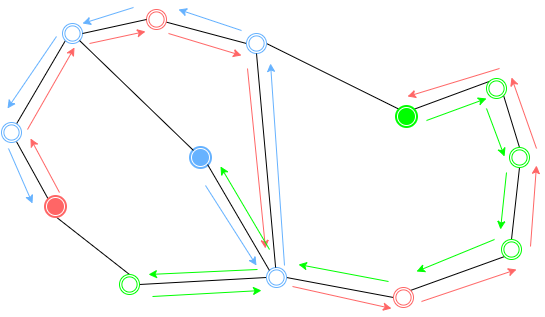
\includegraphics[scale=0.6]{images/Circulartsp.png}

\Section{A probléma megoldása}

A több ügynökös, egy lerakatos utazó ügynök probléma modellje kiszállítási helyzetekre szabva\\

A több ügynökös, egy lerakatos utazó ügynök probléma esetén legyen V a csúcsok halmaza, xi,j az, hogy megy-e az i. pontból út a j. pontba közvetlenül, di,j az i. és j. pont távolsága. Legyen m az ügynökök száma és ezáltal a kapott célfüggvény:

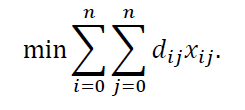
\includegraphics[scale=0.5]{images/mtsp1.png}

Minden pontba csakis egy út indul, kivétel ez alól a 0. pont ami maga az étterem:

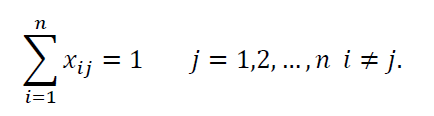
\includegraphics[scale=0.5]{images/mtsp2.png}

Minden pontból csak egy út érkezik, kivétel ez alól a 0. pont ami maga az étterem:

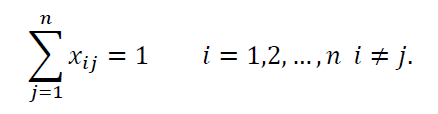
\includegraphics[scale=0.5]{images/mtsp3.png}

Az étteremre való feltétel:

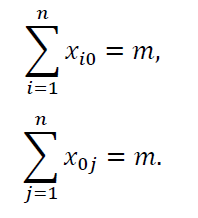
\includegraphics[scale=0.5]{images/mtsp4.png}

MTSP esetén a kövezkező megszorítások szükségessége elengedhetetlen a helyes sorrendmátrix beteljesüléséhez:

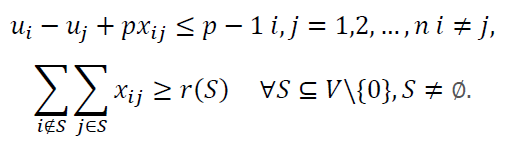
\includegraphics[scale=0.5]{images/mtsp5.png}

A definícióban S a pontok egy részhalmaza, r(S) pedig az, hogy ezt a részthalmazt minimum hány futárnak kell látogatnia. A definíció szumma része megmutatja, hogy minimum hány út megy be a vizsgált pontba. Az éttermet figyelmen kívűl hagyjuk m darab út hagyja el és m darab út megy ki belőle. Ezáltal a fenti egyenlőtlenség nem a futárok tényleges számát adná vissza. 

\Section{A megoldás implementálása}

\Section{A megoldás tesztelése}
